\documentclass[a4paper]{article}

\usepackage[utf8]{inputenc}
\usepackage[T1]{fontenc}
\usepackage{amsmath}
\usepackage{graphicx}
\usepackage{fancyhdr}
\usepackage{tabularx}
\usepackage{hyperref}
\usepackage{etoolbox}% http://ctan.org/pkg/etoolbox
\usepackage{needspace}% http://ctan.org/pkg/needspace

% Für Theoreme (Beispiele, Definitionen, Sätze etc.)
\usepackage{amsthm}

\usepackage[colorinlistoftodos,prependcaption,textsize=tiny]{todonotes}

%\Bearbeitet Format, sodass statt der Einrückung bei Paragraphen durch Zeilenabstand ersetzt wird
\usepackage{parskip}
\setlength\parindent{0pt}

%\Setzt Dokumentinformationen
\title{Master-Thesis: Incremental Analysis of Software Product Lines}
\author{Moritz Fl\"oter}
\date{June 2018}



\begin{document}
\bibliographystyle{unsrt}

\newtheoremstyle{mystyle}% name
  {3pt}%Space above
  {3pt}%Space below
  {\normalfont}%Body font
  {0pt}%Indent amount
  {\bfseries}% Theorem head font
  {}%Punctuation after theorem head
  {\newline}%Space after theorem head 2
  {}%Theorem head spec (can be left empty, meaning 'normal')

\theoremstyle{mystyle}


\newtheorem{req}{REQ}
\newtheorem{subreq}{REQ}[req]
\newtheorem{subsubreq}{REQ}[req]
\AtBeginEnvironment{req}{\Needspace{5\baselineskip}}
\setcounter{req}{0}

\newcommand*{\reqtable}[4]{
\begin{tabular}{ | p{0.15\textwidth} | p{0.79\textwidth} | }
	\hline
	\textit{Priority} & \begin{minipage}[l]{0.79\textwidth}
	\vspace{0.25em}
		#1
	\vspace{0.25em}
	\end{minipage} \\ \hline
	\textit{Source} & \begin{minipage}[l]{0.79\textwidth}
	\vspace{0.25em}
		#2
	\vspace{0.25em}
	\end{minipage}\\ \hline
	\textit{Description} & \begin{minipage}[l]{0.79\textwidth}
	\vspace{0.25em}
		#3
	\vspace{0.25em}
	\end{minipage} \\ \hline
	\textit{Explanation} & \begin{minipage}[l]{0.79\textwidth} 
	\vspace{0.25em}
		#4
	\vspace{0.25em}
	\end{minipage} \\
	\hline
\end{tabular}
}



%\Deckblatt
\maketitle
\newblock

\begin{center}
floeter@uni-hildesheim.de \par
Matrikel-Nr: 236278 \par
Supervisor: \par
Prof. Dr. Klaus Schmid \par
Christian K\"oher
\end{center}

\newpage
\lhead{{}}
\rhead{\leftmark}
\pagestyle{fancy}

\listoftodos[Notes]
\clearpage

%\Inhaltsverzeichnis
\tableofcontents
\newpage
\bibliographystyle{unsrt}

%\Deckblatt
\maketitle
\newpage

\setcounter{page}{1}
\lhead{{}}
\rhead{\leftmark}
\pagestyle{fancy}

\section{Requirements for the Software System}

\begin{req}[Working Base of Incremental Analysis]
	\reqtable
	{Must}  {Interview}
	{The incremental analysis must work based on the current state of a repository and a proposed change}
	{The working base of each incremental analysis is the previous state before a commit/code change. The increment is represented by the change introduced.}
	
	\begin{subreq}[Input Format for Incremental Analysis] \label{req:git-diff}
		\reqtable
		{Must}  {Interview}
		{The input must be a git-diff}
		{The main input for the analysis is a git-diff. This diff represents a changeset that is to be analysed.}
	\end{subreq}
\end{req}


\begin{req}[Filtering of Source Files] \label{req:early-filtering}
\reqtable
	{Must}  {Interview}
	{The set of source files upon which the analysis operates should be reduced to a minimum before being passed to the extractors.}
	{Because extraction is costly, the filtering of source files must happen on a file basis before the extractors are called.}
\end{req}

\clearpage
\begin{req}[Configuration of Filters for Input-Files] \label{req:optimization}
\reqtable
	{Must}  {Initial Description}
	{
	The implemented infrastructure must provide means to configure different filters for the files that are to be analyzed.
    }
	{Depending on the extractor in use and the way it processes input files, different options cover different use cases. Furthermore different filters may affect the overall performance of the software system.}

\begin{subreq}[Implementation of Filters for Input-Files]
    \reqtable
	{Must}  {Interview, Initial Description}
	{
	The filters listed below must be implemented \cite{req:optimization}:
	\begin{itemize}
		\item off \\
		no filtering 
	    \item change only \\
	    only work with files that were modified
	    \item variability-change only \\
	     only work with files where the variability information was changed
	\end{itemize}
    }
	{In order to evaluate different filter methods and their effect on performance, different categories of filtering are required. Off represents the state where no filtering is done, while change performs superficial filtering without regarding variability information directly. The last option analyzing variability change is the most sophisticated filtering option of the three as it requires an analysis of the filecontent of each input file itself.}
\end{subreq}

\begin{subreq}[Implementation of Effect-Filters]
    \reqtable
	{May}  {Interview, Initial Description}
	{
	Of the options listed below must be implemented \cite{req:optimization}:
	\begin{itemize}
		\item change-effect \\
		work with files that were modified and files that were indirectly affected by the change (eg. through includes)
	    \item variability-effect  \\
	    work with files where the variability information was changed and files that were indirectly affected by the variability change
	\end{itemize}
    }
	{When a file is modified, it may affect other files as well that were not changed directly. Consequently, depending on the extractors and analyses used it may be necessary to analyze those files as well.}
\end{subreq}

\end{req}

\begin{req}[Rollback must be possible] \label{req:commit-hook}
\reqtable
	{Must}  {Interview}
	{It must be possible to revert back to the previous state after execution of an incremental analysis.}
	{An Analysis may change the source-files used as input for the extractors along with other changes. Those changes reflect the changes introduced by the new increment that was used as input. If that increment however contains defects identified by the analysis the user might choose to revert the changes and propose an alternative change. This alternative change can only be analyzed if KernelHaven reverts to the original state before the initial change.}

\end{req}

\begin{req}[Dead Code Analysis] 
\reqtable
	{Must}  {Initial Description}
	{The Dead Code Analysis must be integrated in the software system including support for incremental processing}
	{The Dead Code Analyis serves as a practical example for block based analyses. It is used to demonstrate and evaluate the effectiveness of the incremental approach.}
\end{req}

\clearpage
\begin{req}[Target Source File Formats] 
\reqtable
    {Must}  {Initial Description}
	{The software system must support the processing of *.c, *.h, makefile, Kbuild and Kconfig files}
	{The filetypes listed above represent the CodeModel, BuildModel and VariabilityModel of the Linux kernel. As the Linux kernel is used for the evaluation of the implemented incremental analysis approach, those filetypes need to be considered.}
\end{req}

\begin{req}[Analysis Result] 
\reqtable
    {May}  {Interview}
	{The analyis result should only contain elements that resulted of the analyzed increment}
	{As the analysis should provide feedback for the developer on his work, the results should only include elements affected by his work.}
\end{req}

\newpage

\section{Implementation Approaches}

In this section different approaches the integration of incremental analyses will be presented and discussed. Those approaches evolve around KernelHaven using the exisiting infrastructure and implementing additional functionality as extensions or plugins. For remainder of this work, the term "modelset" refers to a set of instances of the Variability-Model, Code-Model and Build-Model.

\subsection{General Approach}

The analysis may be divided into three main phases. In the first phase (preparation-phase), the input for the extractors and analysis is defined while in the second phase (extraction-phase) the extractors run and update the modelset. Finally in the third phase (analysis-phase) the analysis itself is performed.


\subsection{Early Filtering Approach} \label{early}

This approach maintains one version of the modelset. The modelset resulting of the extraction will be based on the version of the modelset that is available from the last run of the analysis. Because unchanged parts of the modelset may be reused from the previous modelset, the extraction process is expected to be less costly than a full extraction of the modelset from scratch.

\subsubsection{How does this work?}

The prepraration phase aims to restrict the set of files that the extractors need to work with to a minimum. In order to achieve that goal, the options specified in REQ \ref{req:optimization}  are integrated. Considering the code model only this would mean the following:

\begin{itemize}
	\item all changed *.c and *.h files
	\item all changed *.c and *.h files along with other files affected by changes in those files (eg. a class using one of the changed classes)
	\item only those *.c and *.h files where the code-model did change
	\item only those *.c and *.h files where the code-model did change along with other files affected by changes in those files
\end{itemize}

The selection of an option that includes indirectly affected files aswell depends on the extractor in use while the option for ignoring files where the variability-information did not change is expected to yield perfomance improvements for any type of extractor. The latter is especially relevant for commits that change artifact specific information only as no extractor exectutions or analyses will be required.

For the Variablity-Model and Build-Model, the existing extractors impose restrictions on the options described for the Code-Model. Those extractors only allow for execution on the entire set of input-files representing the model and do not allow to specify a subset of those files as input. Therefore we will have to run the extraction on the entire set of files as soon as the variability information changed in one of them.

So far the proposed options for filtering input files were agnostic of the analyis that is to be performed after the extraction.

In addition to those options one could consider to filter out variability-changes that are not expected to result in changes for the analysis. For example renaming or deleting a feature would not result in additional dead-code blocks for the dead-code-analysis eventhough technically being a change in variability. The same could be true for the introduction of a new feature that does not depend on other features. This is however not a goal for this work.

After extraction the analysis works with the changes that were not filtered out during the preparation-phase.

\subsubsection{Advantages of this Approach}

The advantage of this approach is that it operates on the source file based diff initially provided as input and does not need to compute more abstract changesets (in contrast to \autoref{late}). Furthermore by filtering the input early on, the amount files used as input for the extractors is reduced. Because the input is filtered before the extraction phase, it does not rely on costly diffs between models.

\subsubsection{Disadvantages of this Approach}

By integrating elements which are not agnostic of the analysis into the preparation phase, a coupling between preparation and analysis is introduced. The analysis-agnostic filtering already depends on the type of input-files. Through adding additional source-file specific filtering-logic for the preparation-phase, we further intensify those dependencies.

Assuming an extractor that generates models from a less common type of input files, we would need to adjust the filtering process to be able to consider the nature of changes within the source-files.

\subsection{Late Filtering Approach} \label{late}

The Late Filtering Approach may only apply the generic change-only filter if applicable for the extractor in quastion during the preparation phase and then starts the extraction-phase. After extraction, the resulting modelset is compared with the previous modelset and changes in variability are determined.

\subsubsection{How does this work?}

Following the ideas outlined in \autoref{early}, we also divide the process into three phases.

After the extraction-phase, the analysis then uses the identified changeset within the modelset to compute its results. As a result of this procedure, artifact specific changes that do not change variability do not get processed by the core-analysis itself - the changeset of the modelset would simply not include any changes in this case. It is now also possible for the analysis to identify the nature of changes within the modelset such as deletion, renaming or addition of a feature.

\subsubsection{Advantages of this Approach}

The advantage of this approach are reduced dependencies between the elements of the three phases. While we can still perform everything proposed in the One Phase Approach, filters may now also be moved to the analyis-phase. We could for example use the same analyis for different extractors running on all changed files and then later identify the differences in the resulting models. Different extractors might be able to handle different types of source-files while the filtering method used is fairly generic. Therfore the possibilities for reuse of an incremental analysis are improved.

Given that KernelHaven creates abstractions of the models represented by source-files through its extractors, pushing analyis-related tasks towards the analysis-phase also falls more in line with the conceptual background of KernelHaven.

\subsubsection{Disadvantages of this Approach}

By using generic or no filters during the preparation phase, the extraction-phase gets more costly. Furthermore computing a diff between two modelsets requires additional computation time.


\clearpage

\section{Software Design}

This section describes the software design and provides reasoning for design decision.

\subsection{State of the KernelHaven Project}

KernelHaven is an infrastructure for analyses on software product lines \cite{KroeherEl-SharkawySchmid18}. This infrastructure will be used and extended to support incremental analyses. 

\autoref{fig:KernelHaven-Architecture} shows the basic architecture of Kernelhaven. Code, Build and VarModel-files are used as input for the extractors which extract the according models that may then be used for analyses. While existing extractors for KernelHaven mostly cover Linux specific input files, it is technically possible to create extractors working on different kinds of input files through a plugin interface.

KernelHaven typically is configured through a configuration-file which is written in the form of a java properties file with no processing of input information happening before the extractors and analysis are started. However it is possible to run preparation tasks before any other elements of the KernelHaven infrastructure are executed.

As KernelHaven follows the style of a pull pipeline, the analysis then may request certain models which are then requested and delivered either from cache or through processing of input files. Analyses may also consist of multiple elements chained after each other or even running in parallel.

\begin{figure}[htbp] 
  \centering
  \begin{minipage}[b]{1\textwidth} 
    \caption[KernelHaven-Architecture]{KernelHaven-Architecture}\label{fig:KernelHaven-Architecture}
    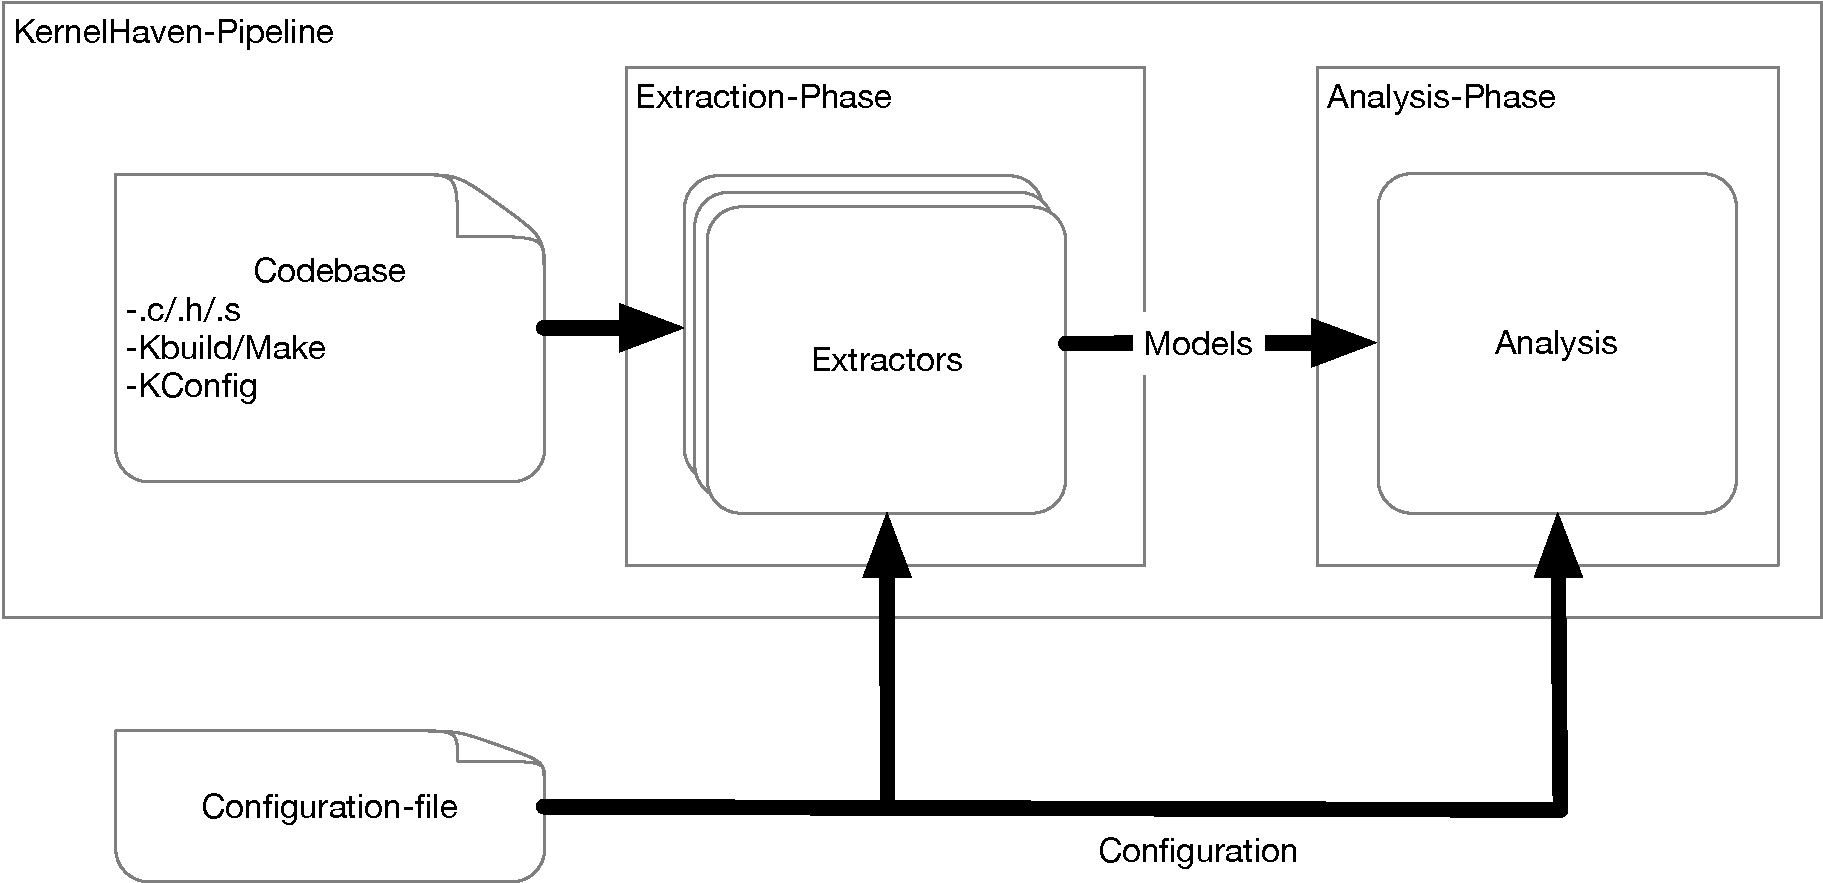
\includegraphics[width=1\textwidth]{img/KernelHaven.pdf}
  \end{minipage}
\end{figure}




\subsection{Decision for the Early Filtering Approach }

After proposing Late Analysis Approach, it became apparant that the assumed performance cost compared to the Early Analysis Approach was estimated as too high to warrant the implementation of this approach. Given that the extraction process itself usually consumes the largest amount of time when performing an analysis without the incremental approach, practical experience supports that decision. The requirement for early filtering is represented in REQ \ref{req:early-filtering}. Therefore the architecture evolves around the Early Filtering Approach.

\subsection{Inclusion of the Early Analysis Approach in KernelHaven}

Following REQ \ref{req:early-filtering} the filtering of data for the analysis is happening in the preparation phase before any of the other components of KernelHaven are run. As the input for an incremental analysis is a git-diff (see REQ \ref{req:git-diff}), the filtering happens based on the changes introduced implementing the options outlined in REQ \ref{req:optimization}.

\begin{figure}[htbp] 
  \centering
  \begin{minipage}[b]{1\textwidth} 
    \caption[KernelHaven-Architecture-Incremental]{KernelHaven-Architecture for Incremental Analyses}\label{fig:KernelHaven-Architecture-Incremental}
    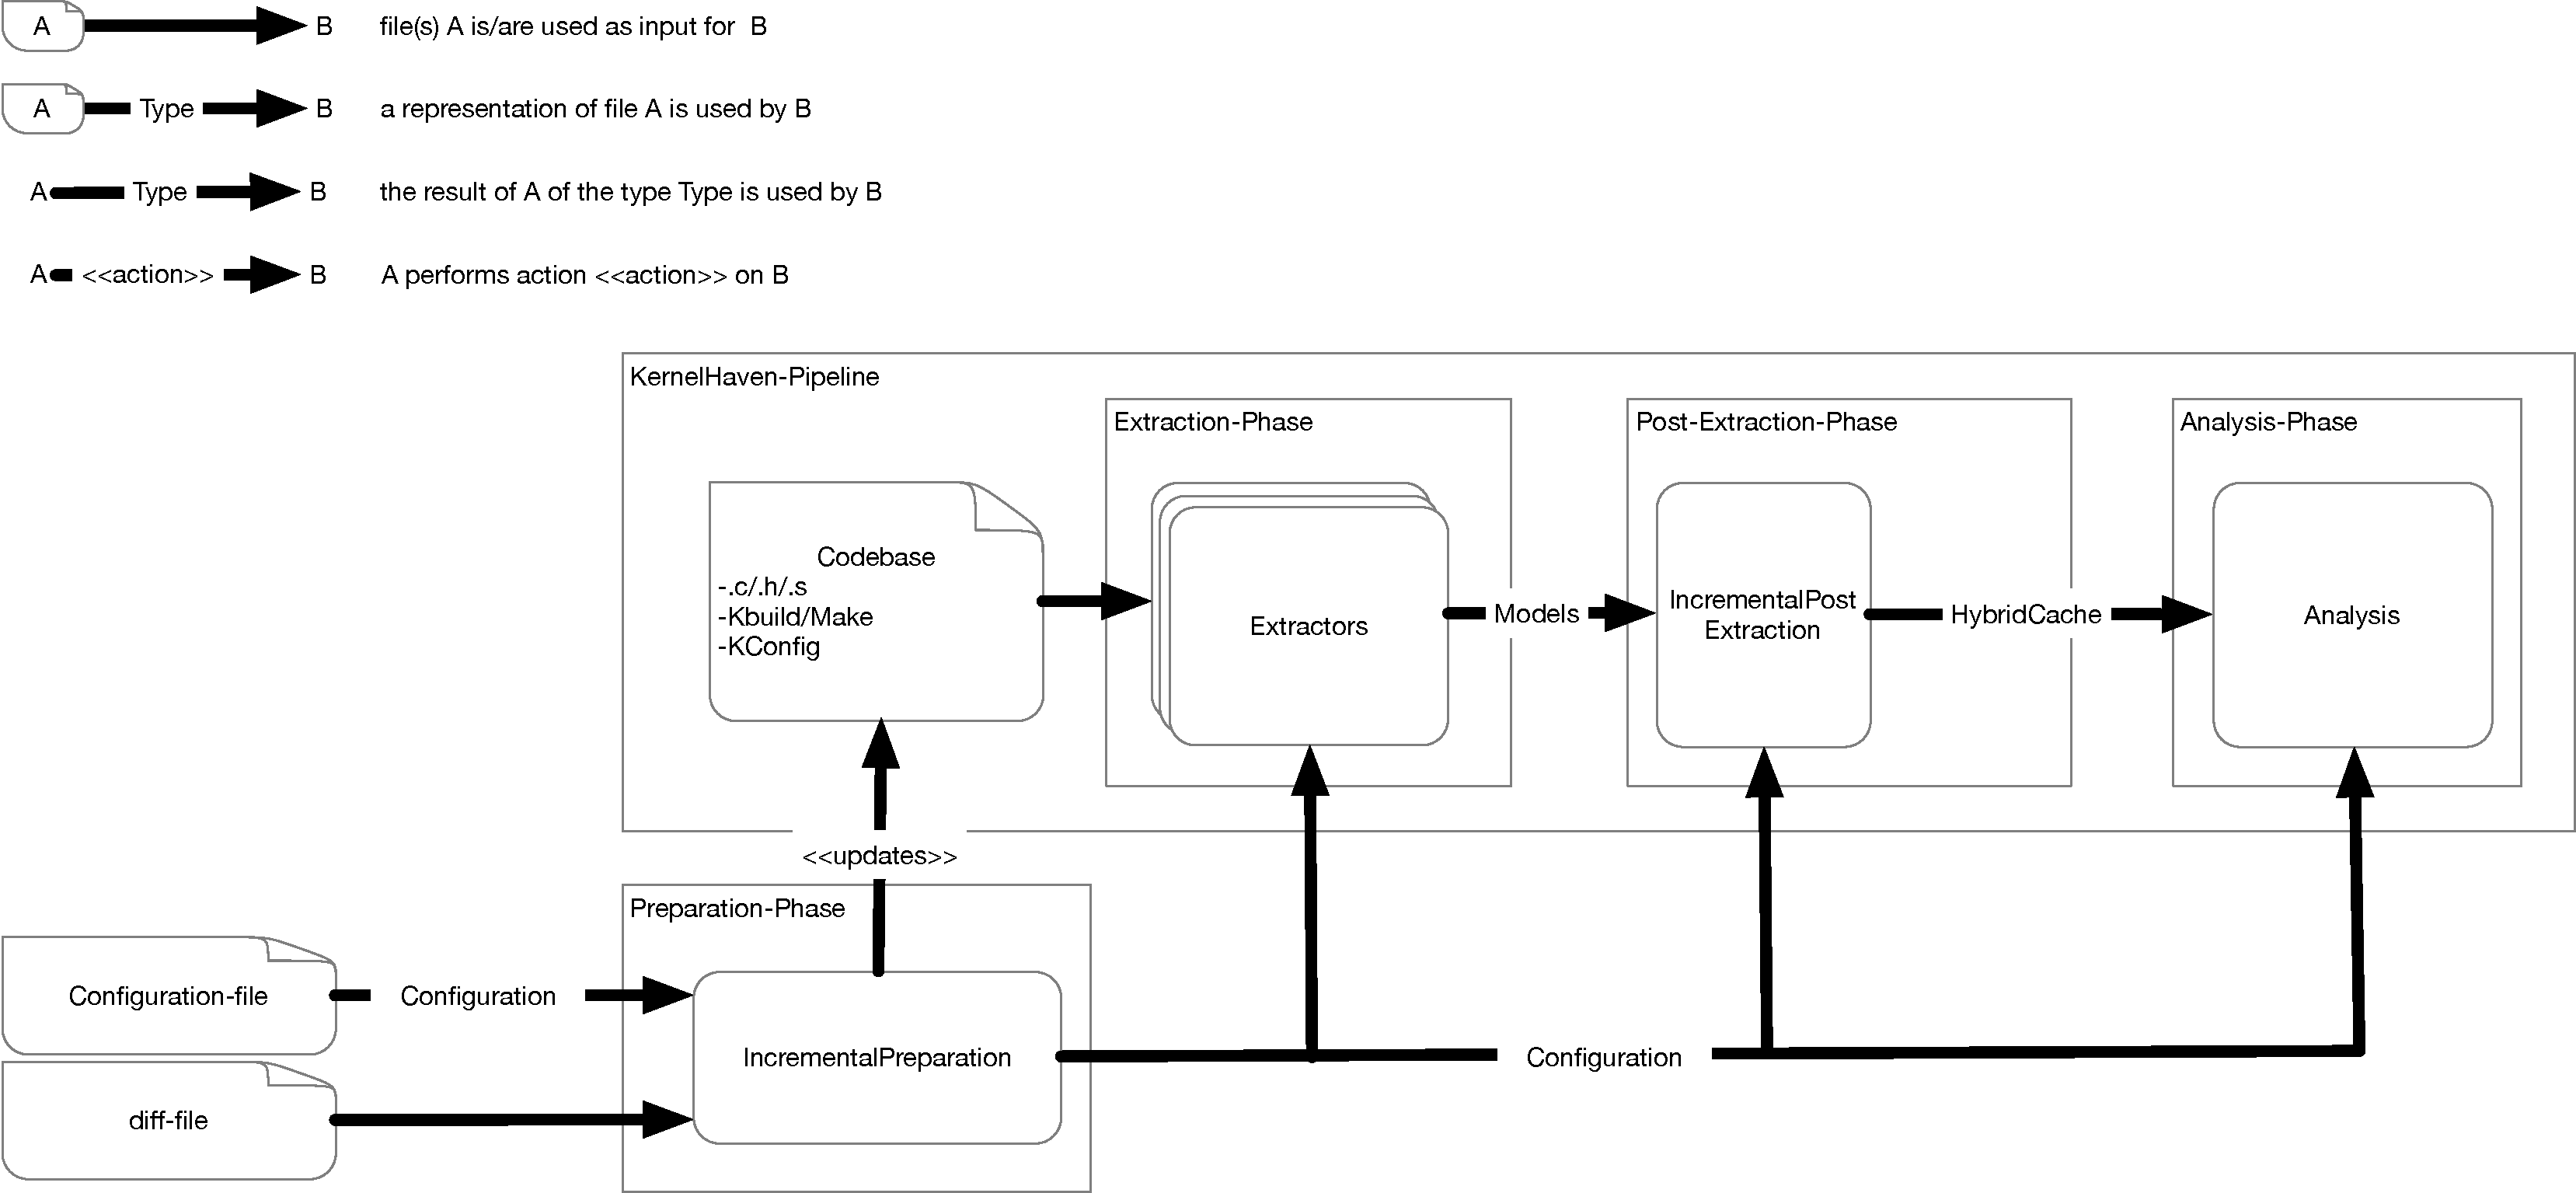
\includegraphics[width=1\textwidth]{img/KernelHavenIncremental.pdf}
  \end{minipage}
\end{figure}

A subset of the most recent source-files including the changes from the git-diff is then used as input for the extractors. After the extractors terminate, the resulting models are stored in a hybrid model cache. This cache differenciates between new files resulting of the current execution and files representing the previous state of the source files but not for any older stages than that. The analyis uses the new files to define on which parts of the models it needs to run reusing unchanged parts of the models from the previous state.

In order to better understand the use of the previous model imagine the following cases:

\begin{itemize}
	\item A git-diff introduces changes to build or varmodel-files only \\
	$\rightarrow$ because those changes may affect all code files, the analysis runs on all CodeModel elements extracted in previous runs
	\item A git-diff introduces changes to code-files only \\
	$\rightarrow$ VarModel and BuildModel did not change but are relevant for a Dead Code Analysis and may be reused
\end{itemize}

After successful execution, the newly extracted parts of the model may be merged with the older models thereby resulting in a set of files that might then be reused in the next iteration of the analysis.

However because the analysis must be able to run in the context of a pre-commit hook (see \ref{req:commit-hook} and the outcome of the analysis might result in a rejection of a commit, it must also be possible to discard newly extracted files and keep the previous model unchanged after the analysis.

\subsection{The Preparation Phase}

In order to provide a set of files to work with for the extractors, a storage for the codebase is used within the incremental analysis. When the git-diff used as input for the incremental analysis introduces changes, those changes get merged on file level with the files currently present in the repository. Subsequently, inputs for the extraction are defined and the analysis gets performed. Depending on the setup of the analysis and whether it is used in the context of a pre-commit-hook that might reject commits, either need to be kept or reverted.

\begin{figure}[htbp] 
  \centering
  \begin{minipage}[b]{1\textwidth} 
    \caption[Preparation-Phase Overview]{Preparation-Phase Overview}\label{fig:preparation-overview}
    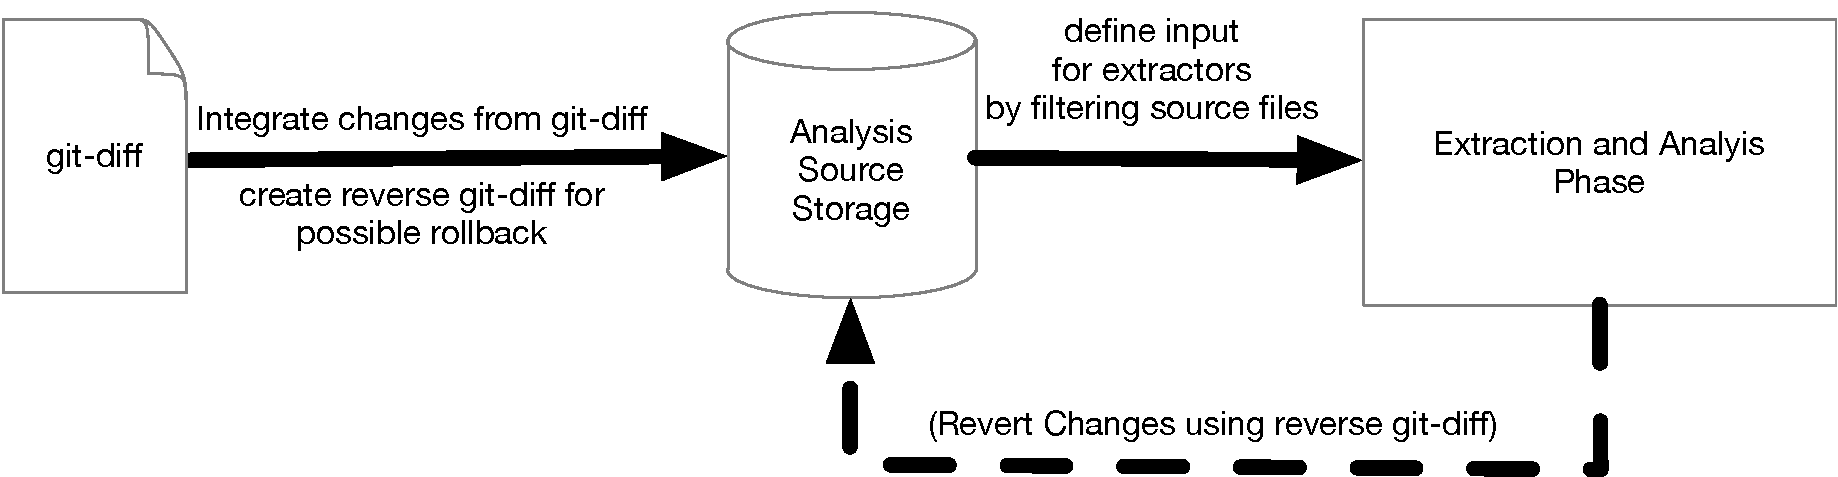
\includegraphics[width=1\textwidth]{img/PreparationOverview.pdf}
  \end{minipage}
\end{figure}

The choice for a storage system representing source files as they exist in the source repo on the level of the filesystem stems from the way current extractors handle their input. Those extractors operate based on the filesystems and are started through calls to command line interfaces. It is therefore not possible to implement access to relevant information through an abstraction. Therefore we require a solution that provides the input-files based on the file-system.

The approach to simply maintain two different folders for the previous and current version of the source-files is  not feasible as this would require time-consuming copying of the source-files from the previous version in order to create a folder containing the source-files including the changes described through the git-diff. Furthermore storage requirements would be doubled. Storage requirements are also the reason for discarding git as a system to manage rollbacks as the history building up in that repository would require additional storage space.

Therefore we rely on a reverse git diff for rollbacks on top of a flat file system. The reverse git-diff basically is a diff describing the changes from the merged result to the original set of source files. The generation of this reverse diff could be managed by reversing the changes introduced by the input-diff - an addition becomes a deletion, a deletion becomes an addition. However for early implementations one could also rely on the diff being provided externally for example through the creation of those two diffs within the pre-commit hook.

After changes are integrated, the relevant inputs for the extractors are defined based on the git-diff and working on the files present in the local source-file repository. The result of the analysis and the configuration settings determine whether the changes need to be commited to the analysis repository or may in fact be reverted. A reversion of the changes is required whenever the incremental analysis is executed in the context of a pre-commit-hook and the corresponding commit does not get merged with the main developer-repository.

\subsection{The Extraction Phase}

The main component added to the extraction phase is the Hybrid Cache. This cache contains up to two most versions of the modelset but never more than that.

After the extractors are called on a subset of the code source, the result is a subset of the all model elements describing the code source. Because the extractors only run on files that require extraction, the new extractor results can be regarded together with the previous modelset effectively replacing any files that were already present in that set. So in order to gain a representation of the entire modelset after integrating the proposed change defined through the git-diff, one prioritizes the usage of newly extracted model-files but uses the old model-files whenever there is a corresponding new model-file present.

As we might require a rollback if a proposed change is rejected, we can not simply overwrite the existing model-files with the new ones. However because KernelHaven-Analyses are written in Java, we can implement access to the Hybrid Cache through a Java classes - this was not possible for the source files repository of the analysis because of the outlined restrictions for the extractors.

To understand the setup of the HybridCache, we first look at the existing cache. The existing cache in KernelHaven writes files to a folder. Each code-file is represented as a single model-file in the cache while variability and build information both are stored in a single file. The names of the code-model-files correspond to the names of the code-files used as extractor input - the same code-file will always result in a code-model-file with the same name. After the extractors run, the extracted models may be written to the cache as model-files.

We use two folders for representing the Hybid Cache. One folder contains the previously extracted model-files, while the other is where all newly extracted model-files are written to after extraction. Working with the folder-structure, a Java class enabling access to the models can be created. For accessing the new model it works following the mechanic outlined at the beginning of this subsection. It is however also technically possible to access the old model by using the old model folder exclusively. This opens up the option to revisit the Late Filtering Approach in subsequent work. Depending on the outcome of the analysis and whether a rollback is requested, the files resulting of the most recent extraction are either wiped or merged with the existing model to allow for subsequent iterations of the analysis.

\subsection{Integration with a Pre-Commit Hook}

Using a pre-commit-hook, the git-diff is provided for the analysis. The analysis then is triggered from the hook based on the git-diff, its internal source-files and configuration that defines which extractors to use and whether or not to rollback after new defects are found. Its results of the analysis are then used by the pre-commit hook resulting in either a rejection or acceptance of the commit. While the rejection of a commit might not be feasible for many environments at least a warning should be provided to the developer in case new defects were introduced through his work. This depends mainly on the context and policies in conjunction of which the incremental analysis is used. \todo{Should the rollback be triggered externally or is the kernelhaven-configuration-file ok? or should the commit-hook use policies defined by KernelHaven for rejection or acceptance of commits?}

\begin{figure}[htbp] 
  \centering
  \begin{minipage}[b]{1\textwidth} 
    \caption[Integration with a Pre-Commit Hook]{Integration with a Pre-Commit Hook}\label{fig:pre-commit}
    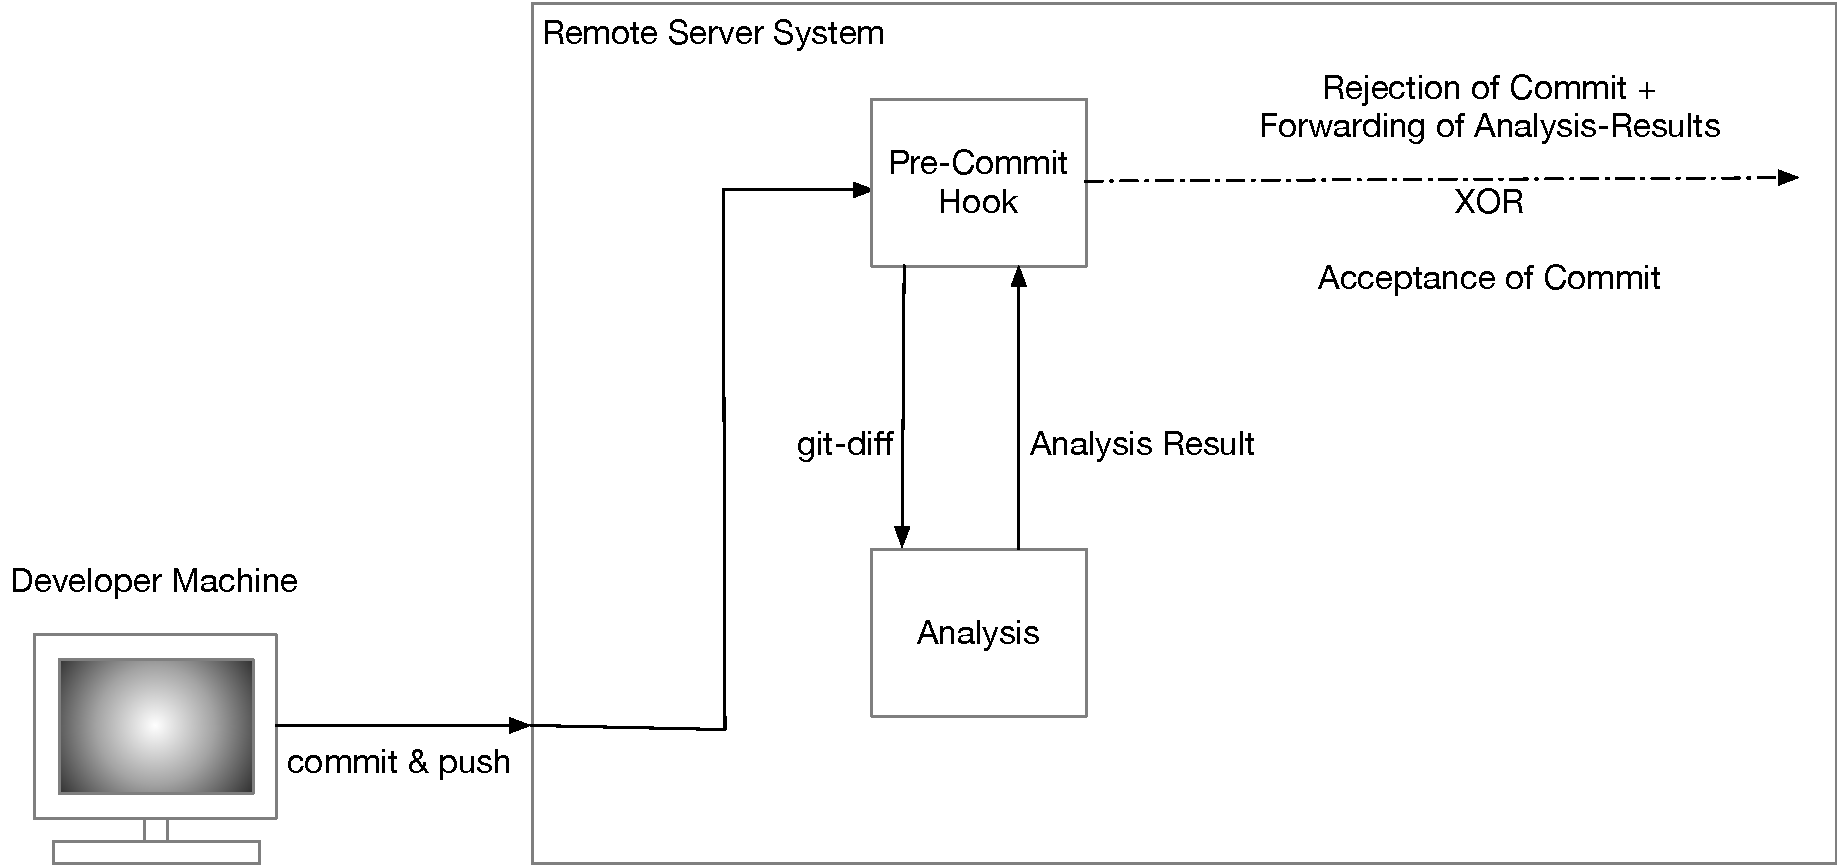
\includegraphics[width=1\textwidth]{img/IntegrationPreCommitHook.pdf}
  \end{minipage}
\end{figure}





%\Bibliography
\newpage

\bibliography{sources}


\end{document}